In this model, each component gets to be a class in its own \verb|.h| (c++) file handling the logic specific for that component in two primary methods; an event polling-method, usually \verb|Read()|, and a time-step method \verb|Update()|. 
The main \verb|.ino| file is responsible for polling each components eventlistener, and calling their appropriate reactive methods (such as activating a pop-bumper, turning an LED on etc.). 
Main repeatedly calls \verb|Update()| in the primary Arduino loop.
In essence, every component becomes a state-machine with \verb|Update()| as its step-function. 
An example snippet from \verb|Main.ino| is shown in \ref{code:main}.
The full structure of the codebase is shown in \ref{fig:codediag}. 

\begin{figure*}
	\begin{lstlisting}[style=c]
  #include "Popbumper.h"
  #include "Flipper.h"
	... // All the subcomponents are brought in here.
	
  // ----- Pin definitions -----
  #define POP1 3      
	... // All used pins are defined here for easy rewiring.
	
  // ----- Global variables -----
  unsigned long score;  // Address passed as argument to each point-giving component
	
  Flipper flipperLeft(BTN_L, FLIP_L);
  Flipper flipperRight(BTN_R, FLIP_R);
  Popbumper bumper1(&score, TAPE1, POP1);
  ... // More imported components are defined here.
	
  // ----- Primary code -----
  void loop() {
		update();
		if(bumper1.IsHit()) { bumper1.Activate(); }
		if(bumper2.IsHit()) { bumper2.Activate(); }
		... // Poll each event-listener function of the subcomponents.
  }
	
  void update() {
 		flipperLeft.Update();
		flipperRight.Update();
		bumper1.Update();
		... // All time-sensitive components are updated at each loop-iteration.
  }
	\end{lstlisting}
	\caption{A snippet of the structure of the main Arduino sketch.}
	\label{code:main}
\end{figure*}


\begin{figure*}[h]
	\centering
	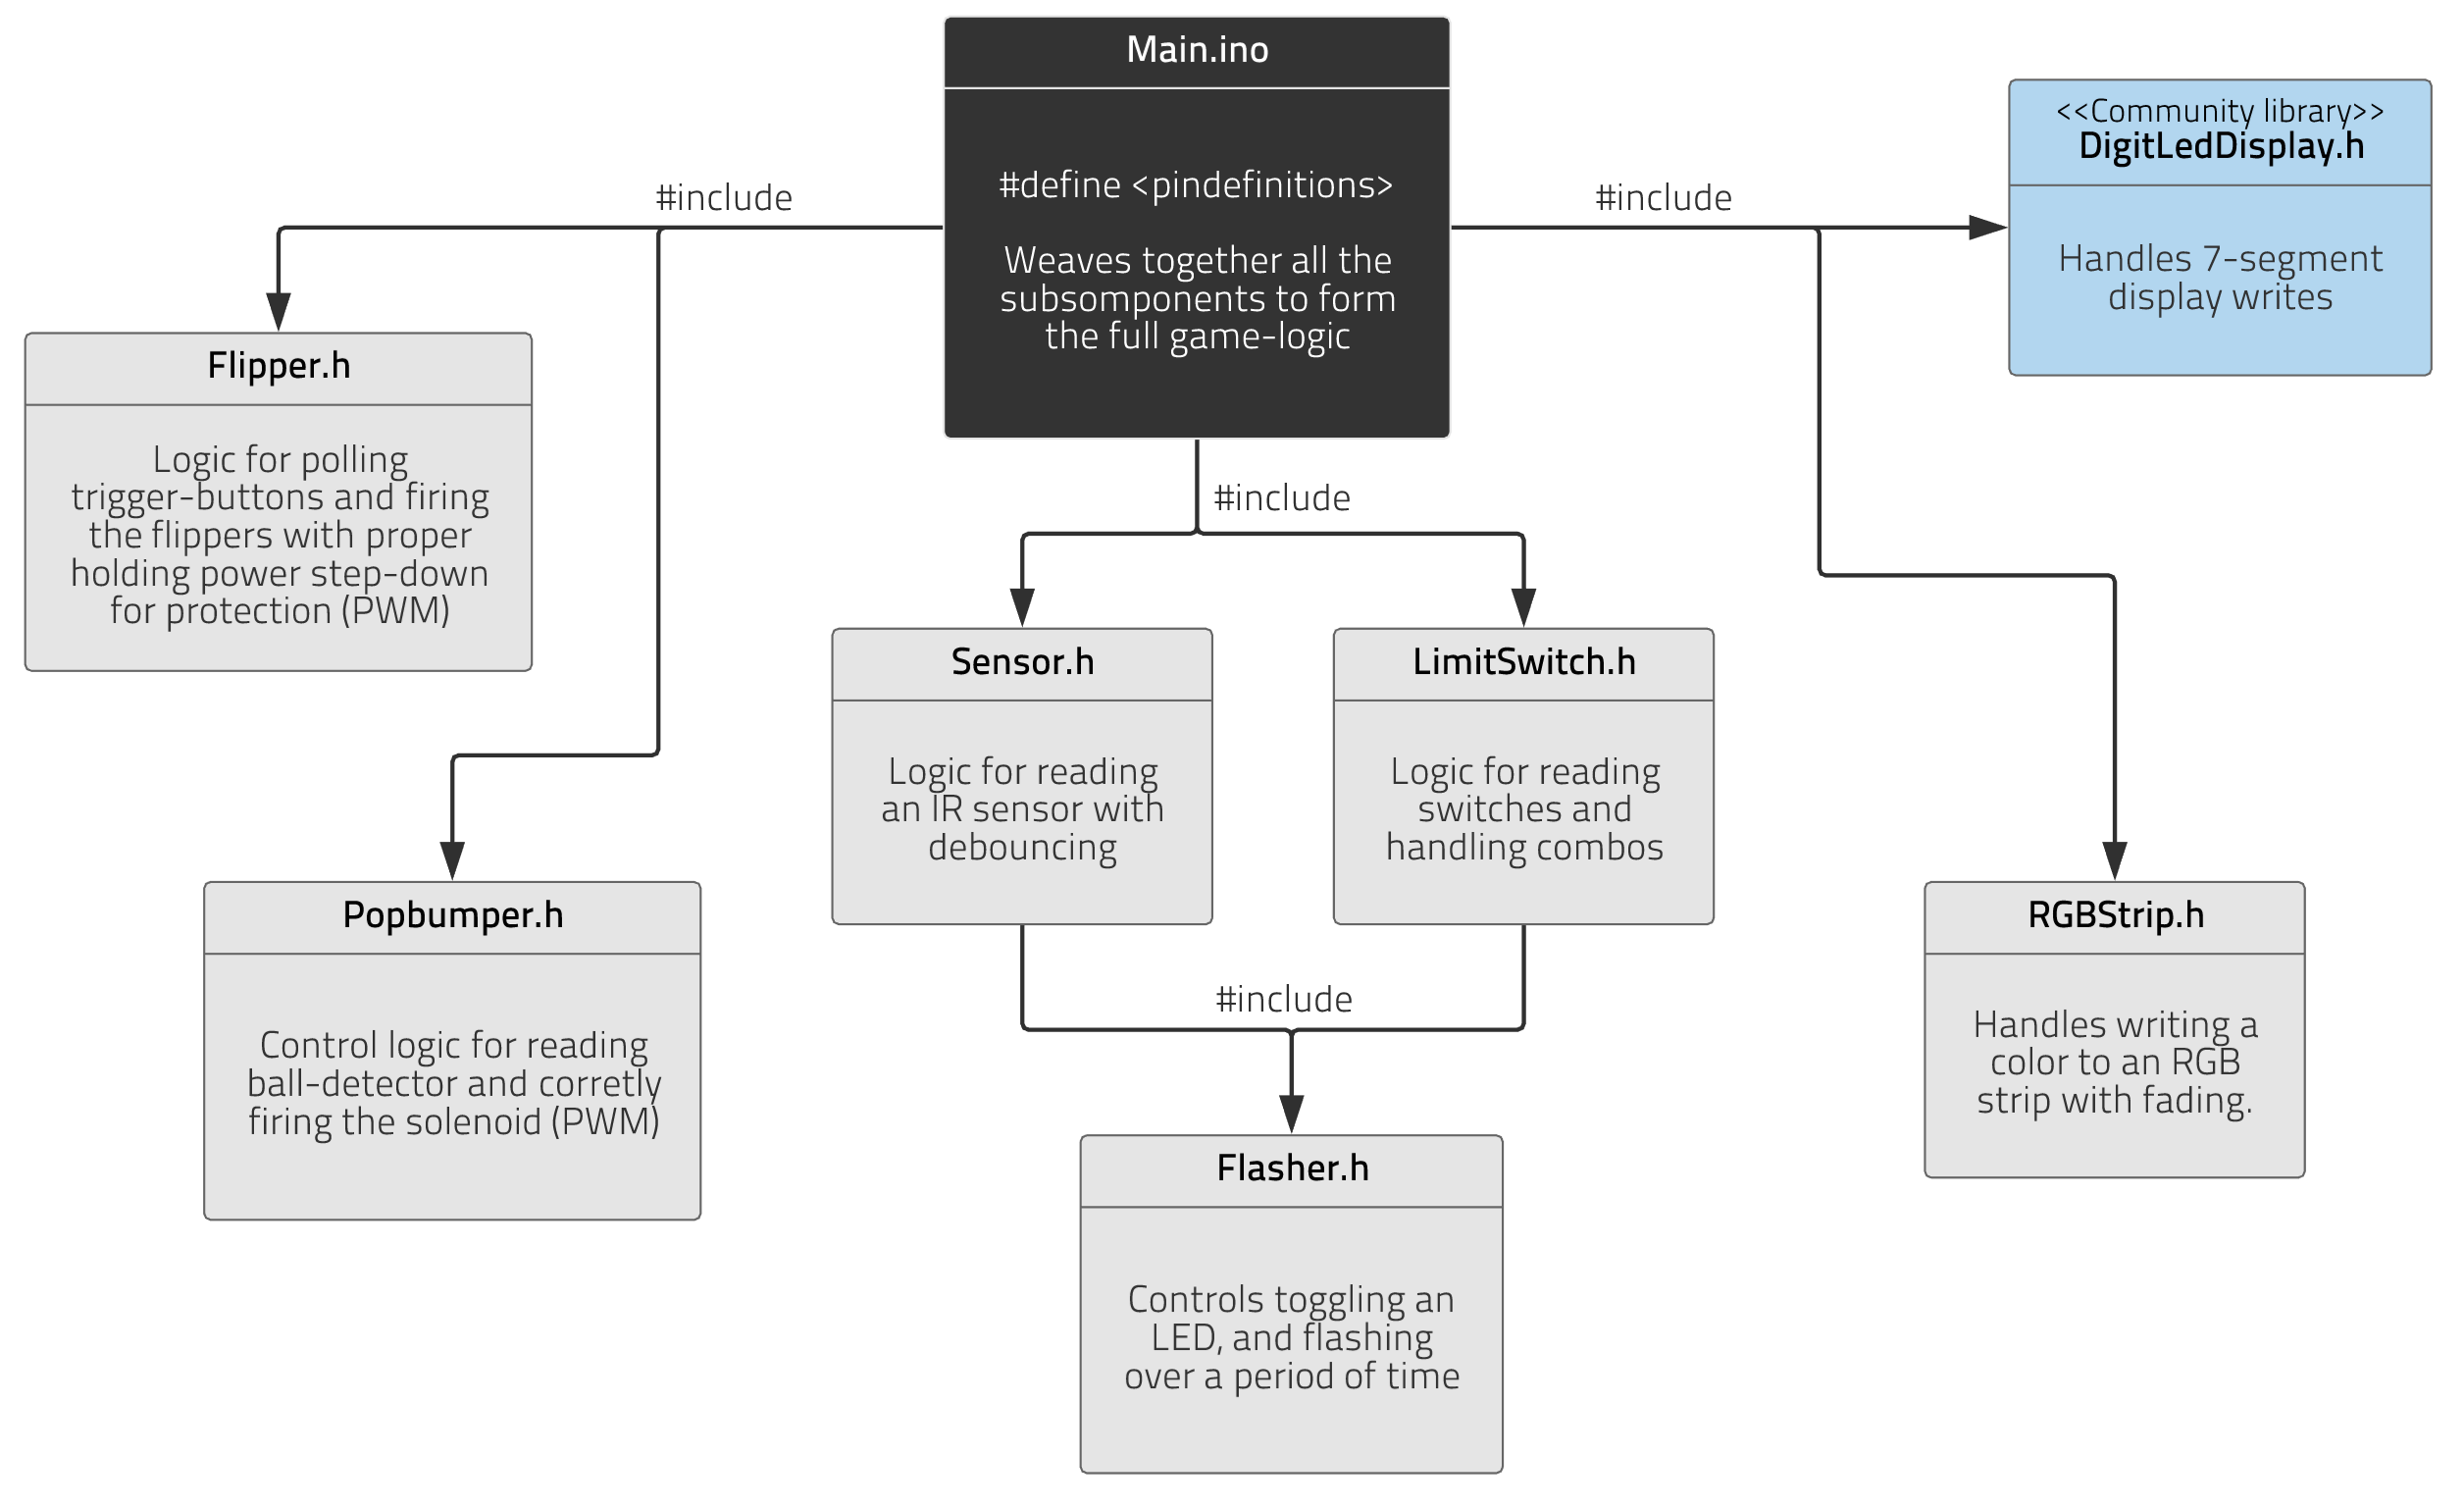
\includegraphics[width=\textwidth]{code_diag}
	\caption{Overview of the code hierarchical structure.}
	\label{fig:codediag}
\end{figure*}